\documentclass[a4paper,12pt,oneside]{book}

%-------------------------------Start of the Preable------------------------------------------------
\usepackage[english]{babel}
\usepackage{blindtext}
%packagr for hyperlinks
\usepackage{hyperref}
\hypersetup{
    colorlinks=true,
    linkcolor=blue,
    filecolor=magenta,      
    urlcolor=cyan,
}

\urlstyle{same}
%use of package fancy header
\usepackage{fancyhdr}
\setlength\headheight{26pt}
\fancyhf{}
%\rhead{
\includegraphics[width=1cm]{logo}}
\lhead{\rightmark}
\rhead{
\includegraphics[width=1cm]{logo}}
\fancyfoot[RE, RO]{\thepage}
\fancyfoot[CE, CO]{\href{http://www.e-yantra.org}{www.e-yantra.org}}

\pagestyle{fancy}

%use of package for section title formatting
\usepackage{titlesec}
\titleformat{\chapter}
  {\Large\bfseries} % format
  {}                % label
  {0pt}             % sep
  {\huge}           % before-code
 
%use of package tcolorbox for colorful textbox
\usepackage[most]{tcolorbox}
\tcbset{colback=cyan!5!white,colframe=cyan!75!black,halign title = flush center}

\newtcolorbox{mybox}[1]{colback=cyan!5!white,
colframe=cyan!75!black,fonttitle=\bfseries,
title=\textbf{\Large{#1}}}

%use of package marginnote for notes in margin
\usepackage{marginnote}
\usepackage{tabularx}
%use of packgage watermark for pages
%\usepackage{draftwatermark}
%\SetWatermarkText{
\includegraphics{logo}}
\usepackage[scale=2,opacity=0.1,angle=0]{background}
\backgroundsetup{
contents={
\includegraphics{logo}}
}

%use of newcommand for keywords color
\usepackage{xcolor}
\newcommand{\keyword}[1]{\textcolor{red}{\textbf{#1}}}

%package for inserting pictures
\usepackage{graphicx}

%package for highlighting
\usepackage{color,soul}

%new command for table
\newcommand{\head}[1]{\textnormal{\textbf{#1}}}


%----------------------End of the Preamble---------------------------------------


\begin{document}

%---------------------Title Page------------------------------------------------
\begin{titlepage}
\raggedright
{\Large eYSIP2017\\[1cm]}
{\Huge\scshape\centering Distributed robotics - multi swarm robots \\[.1in]}
\vfill
\hfill\\
\begin{figure}[h!]
	\centering\includegraphics[width=350px]{./Small_bots.jpg}		
	\caption{A picture of the swarm robots!}
\end{figure}	
\hfill\\
\begin{flushright}
{\large Intern 1 Mr. Chinmay C \\}
{\large Intern 2 Mr. R Hariharan \\}
{\large Mentor 1 Ms. Rutuja \\}
{\large Mentor 2 Ms. Deepa \\}
{\large Duration of Internship: $ 22/05/2017-07/07/2017 $ \\}
\end{flushright}

{\itshape 2017, e-Yantra Publication}
\end{titlepage}
%-------------------------------------------------------------------------------

\tableofcontents

\chapter[Distributed robotics - multi swarm robots]{Distributed robotics - multi swarm robots}
\section{Abstract}
Swarm robotics is a field in robotics which implements coordination of multi robot systems which consist of large number of robots having simpler robots. There is a collective behavior that emerges from interactions between robots and interactions of robots with the environment. This behavior is emerged from field of biological studies of fishes, birds, ants, insects, etc. Application of swarm robotics varies from military, aviation to collective behavior of self driving cars. The objective of the project was to build miniaturized swarm bots and develop an algorithm for generic shape formation.

\subsection*{Following points are completed:}
\begin{itemize}
\item Study the concepts of swarm robotics and get familiar
with different robots available \\
\item Study the kinematics of differential drive configuration \\
\item Selecting appropriate sensors to be added \\
\item Designing the PCB \\
\item Assembling all the components \\
\item Making of Mini bots \\
\item Testing of Mini bots\\
\item Implementing of circle formation of asynchronous fat robots with limited visibility in V-REP simulator\\
\item Developed and implemented generic shape formation algorithm for a system of distributed robots in V-REP simulator\\
\item Implemented follow the leader swarm behavior on Mini bots\\
\item Implemented rendezvous swarm behavior on firebird V robots\\
\end{itemize}

\chapter[Hardware parts]{Hardware parts}
\begin{itemize}
  \item List of hardware: \href{./COMPONENT LIST}{COMPONENT LIST},
  \item Detail of each hardware: Atmega16 \href{./datasheet/atmega16.pdf}{Datasheet}, {Chip component, Lamington road, Mumbai}, 
  \item Detail of each hardware: CD40106 \href{./datasheet/CD40106.pdf}{Datasheet}, {Chip component, Lamington road, Mumbai}, 
  \item Detail of each hardware: L293D \href{./datasheet/L293.pdf}{Datasheet}, {GALA Electronics, Lamington road, Mumbai}, 
  \item Detail of each hardware: LM158 \href{./datasheet/lm158-n.pdf}{Datasheet}, {Chip component, Lamington road, Mumbai}, 
  \item Connection diagram
\end{itemize}
\begin{tabular}{p{0.25\linewidth} p{0.25\linewidth} p{0.25\linewidth} p{0.25\linewidth}}
	\begin{figure}
		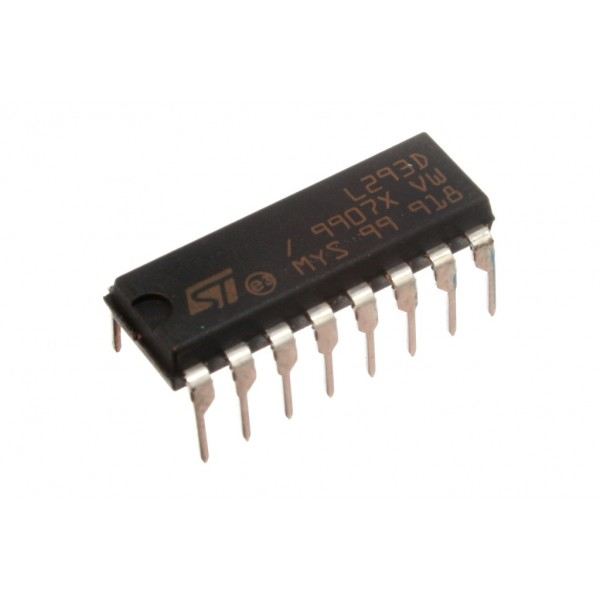
\includegraphics[width=10px]{./l293d.jpeg}		
		\caption{l293d}
	\end{figure} & sdhljkfhs & jsdhfkjsld & jshldfhsdf\\
\end{tabular}
\chapter[Softwares used]{Softwares used}
\begin{itemize}
  \item List of softwares used are V-rep, Fusion 360, AvrDude, Avrgcc, Texstudio, Git 
  \item Details of software: V-rep: 3.4.0, \href{http://www.coppeliarobotics.com/}{download link}, 
  \item Installation steps \href{http://www.coppeliarobotics.com/resources.html}{download link},
  \item Details of software: Fusion 360: 3.4.0, \href{https://www.autodesk.com/products/fusion-360/students-teachers-educators}{download link},
  \item Installation steps \href{https://www.autodesk.com/products/fusion-360/students-teachers-educators}{download link},
  \item Details of software: AvrDude, \href{http://www.nongnu.org/avrdude/}{download link},
  \item Details of software: Avrgcc, \href{https://gcc.gnu.org/wiki/avr-gcc}{download link},
  \item Details of software: texstudio, \href{http://www.texstudio.org/}{download link},
  \item Installation steps \href{http://www.texstudio.org/}{download link},
  \item Details of software: git, \href{https://git-scm.com/}{download link},
  \item Installation steps \href{https://git-scm.com/}{download link},
\end{itemize}

\newpage

\chapter{Assembly of hardware}
Circuit diagram and Steps of assembly of hardware with pictures for each step


\section{Circuit Diagram}
Circuit schematic, simplified circuit diagram , block diagram of system
\hfill\\
\begin{figure}[h!]
	\caption{Back part of pcb}
	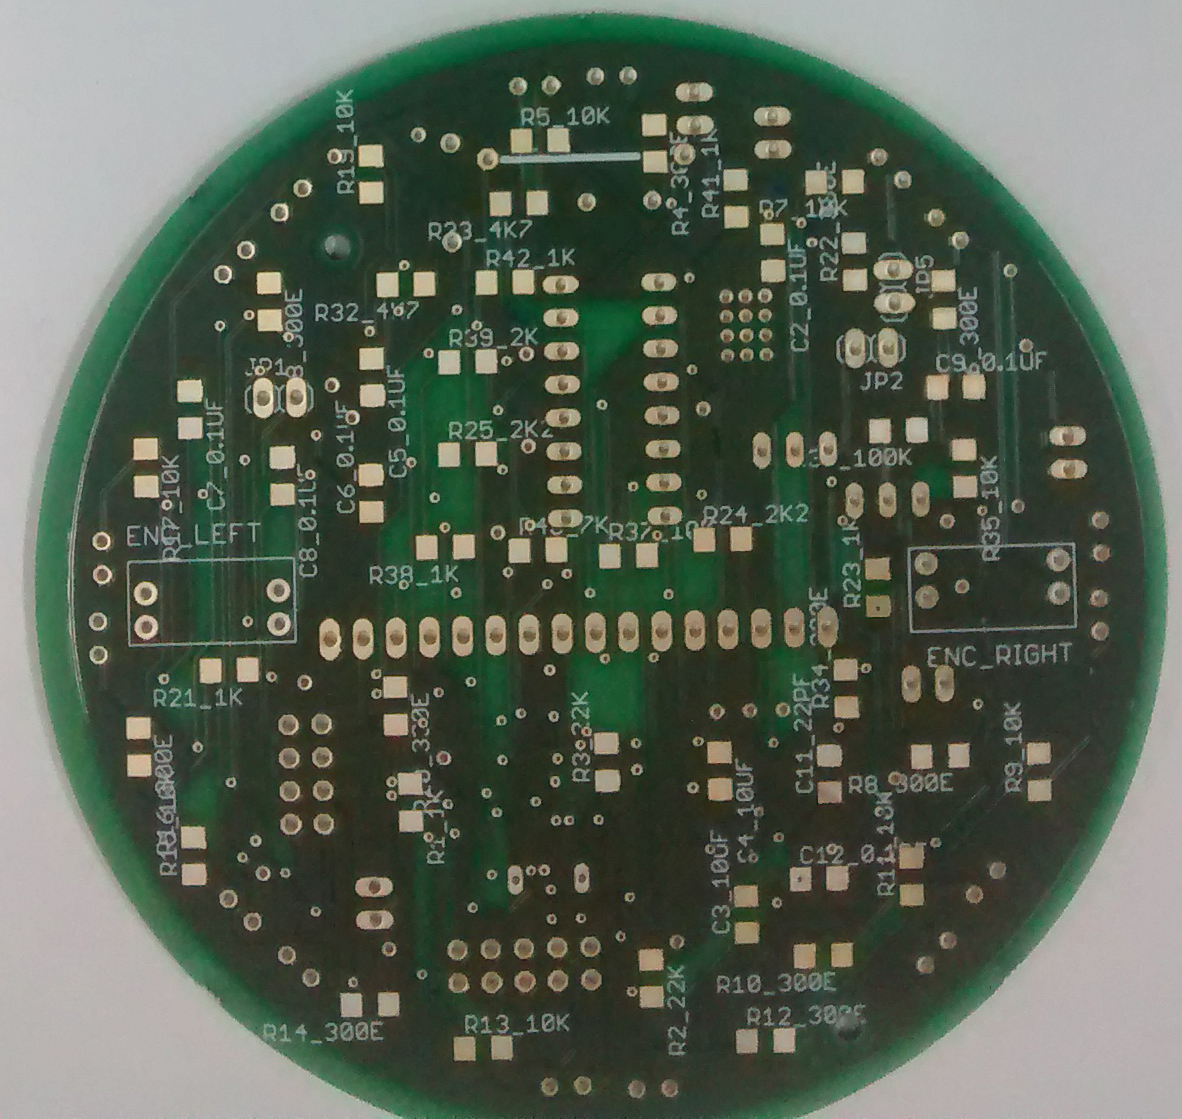
\includegraphics[width=\textwidth]{./Pictures/PCB_back}		
\end{figure}	
\hfill\\
\subsection*{Step 1}
Designing schematics and routing layout of PCB and getting them printed.
\hfill\\
\begin{figure}[h!]
	\caption{Front part of pcb}
	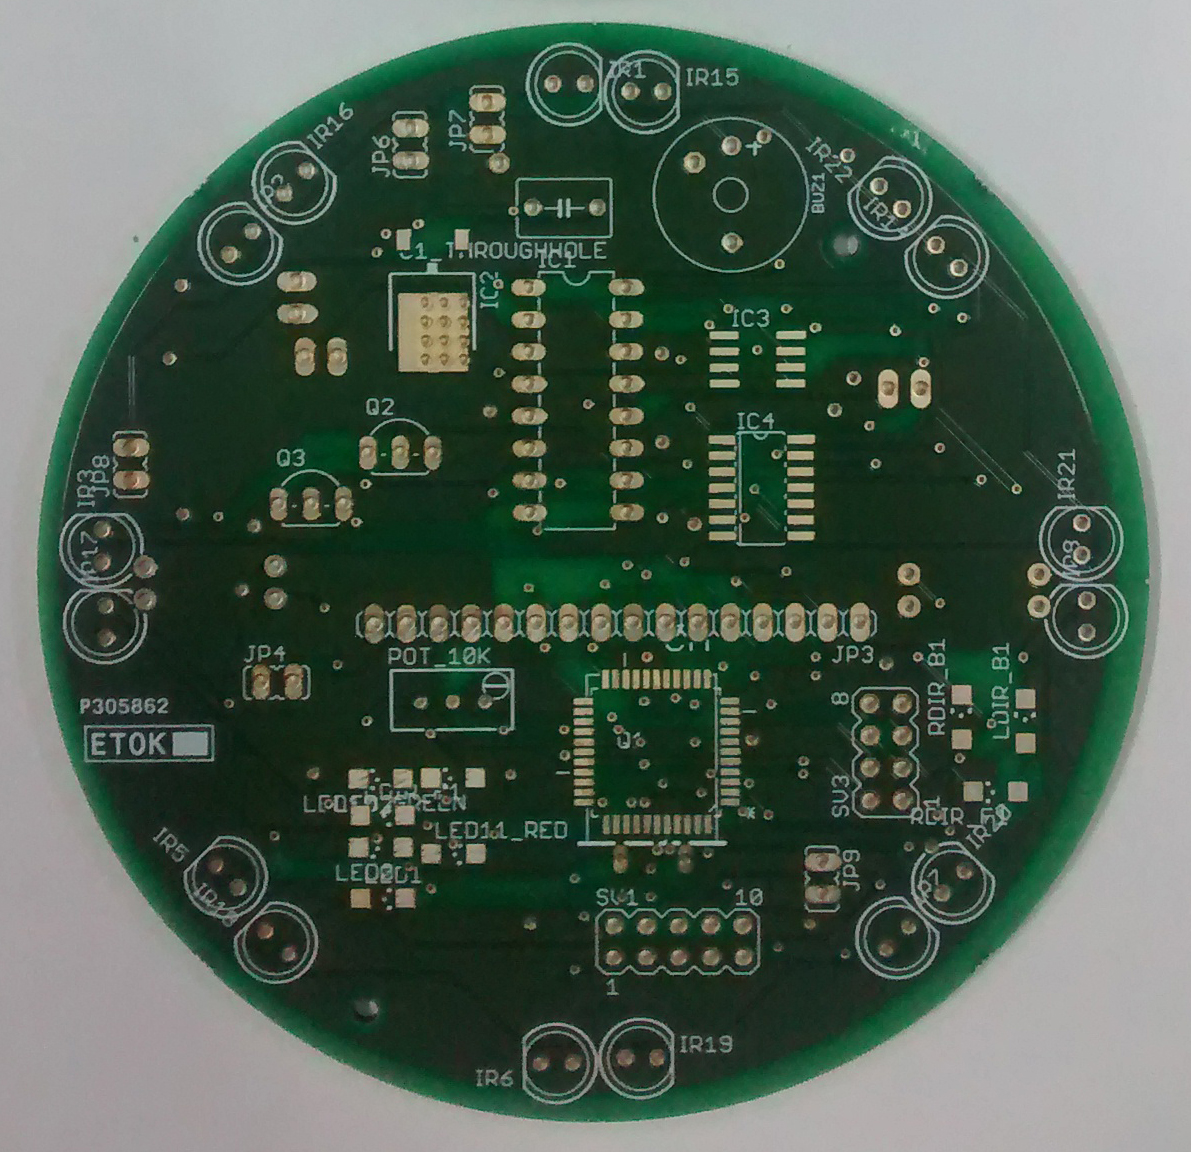
\includegraphics[width=\textwidth]{./Pictures/PCB_front}		
\end{figure}	
\hfill\\
\newpage
\subsection*{Step 2}
Designing chassis and getting them laser cut. Fixing motors with L-clamps 
\hfill\\
\begin{figure}[h!]
	\caption{Chassi design}
	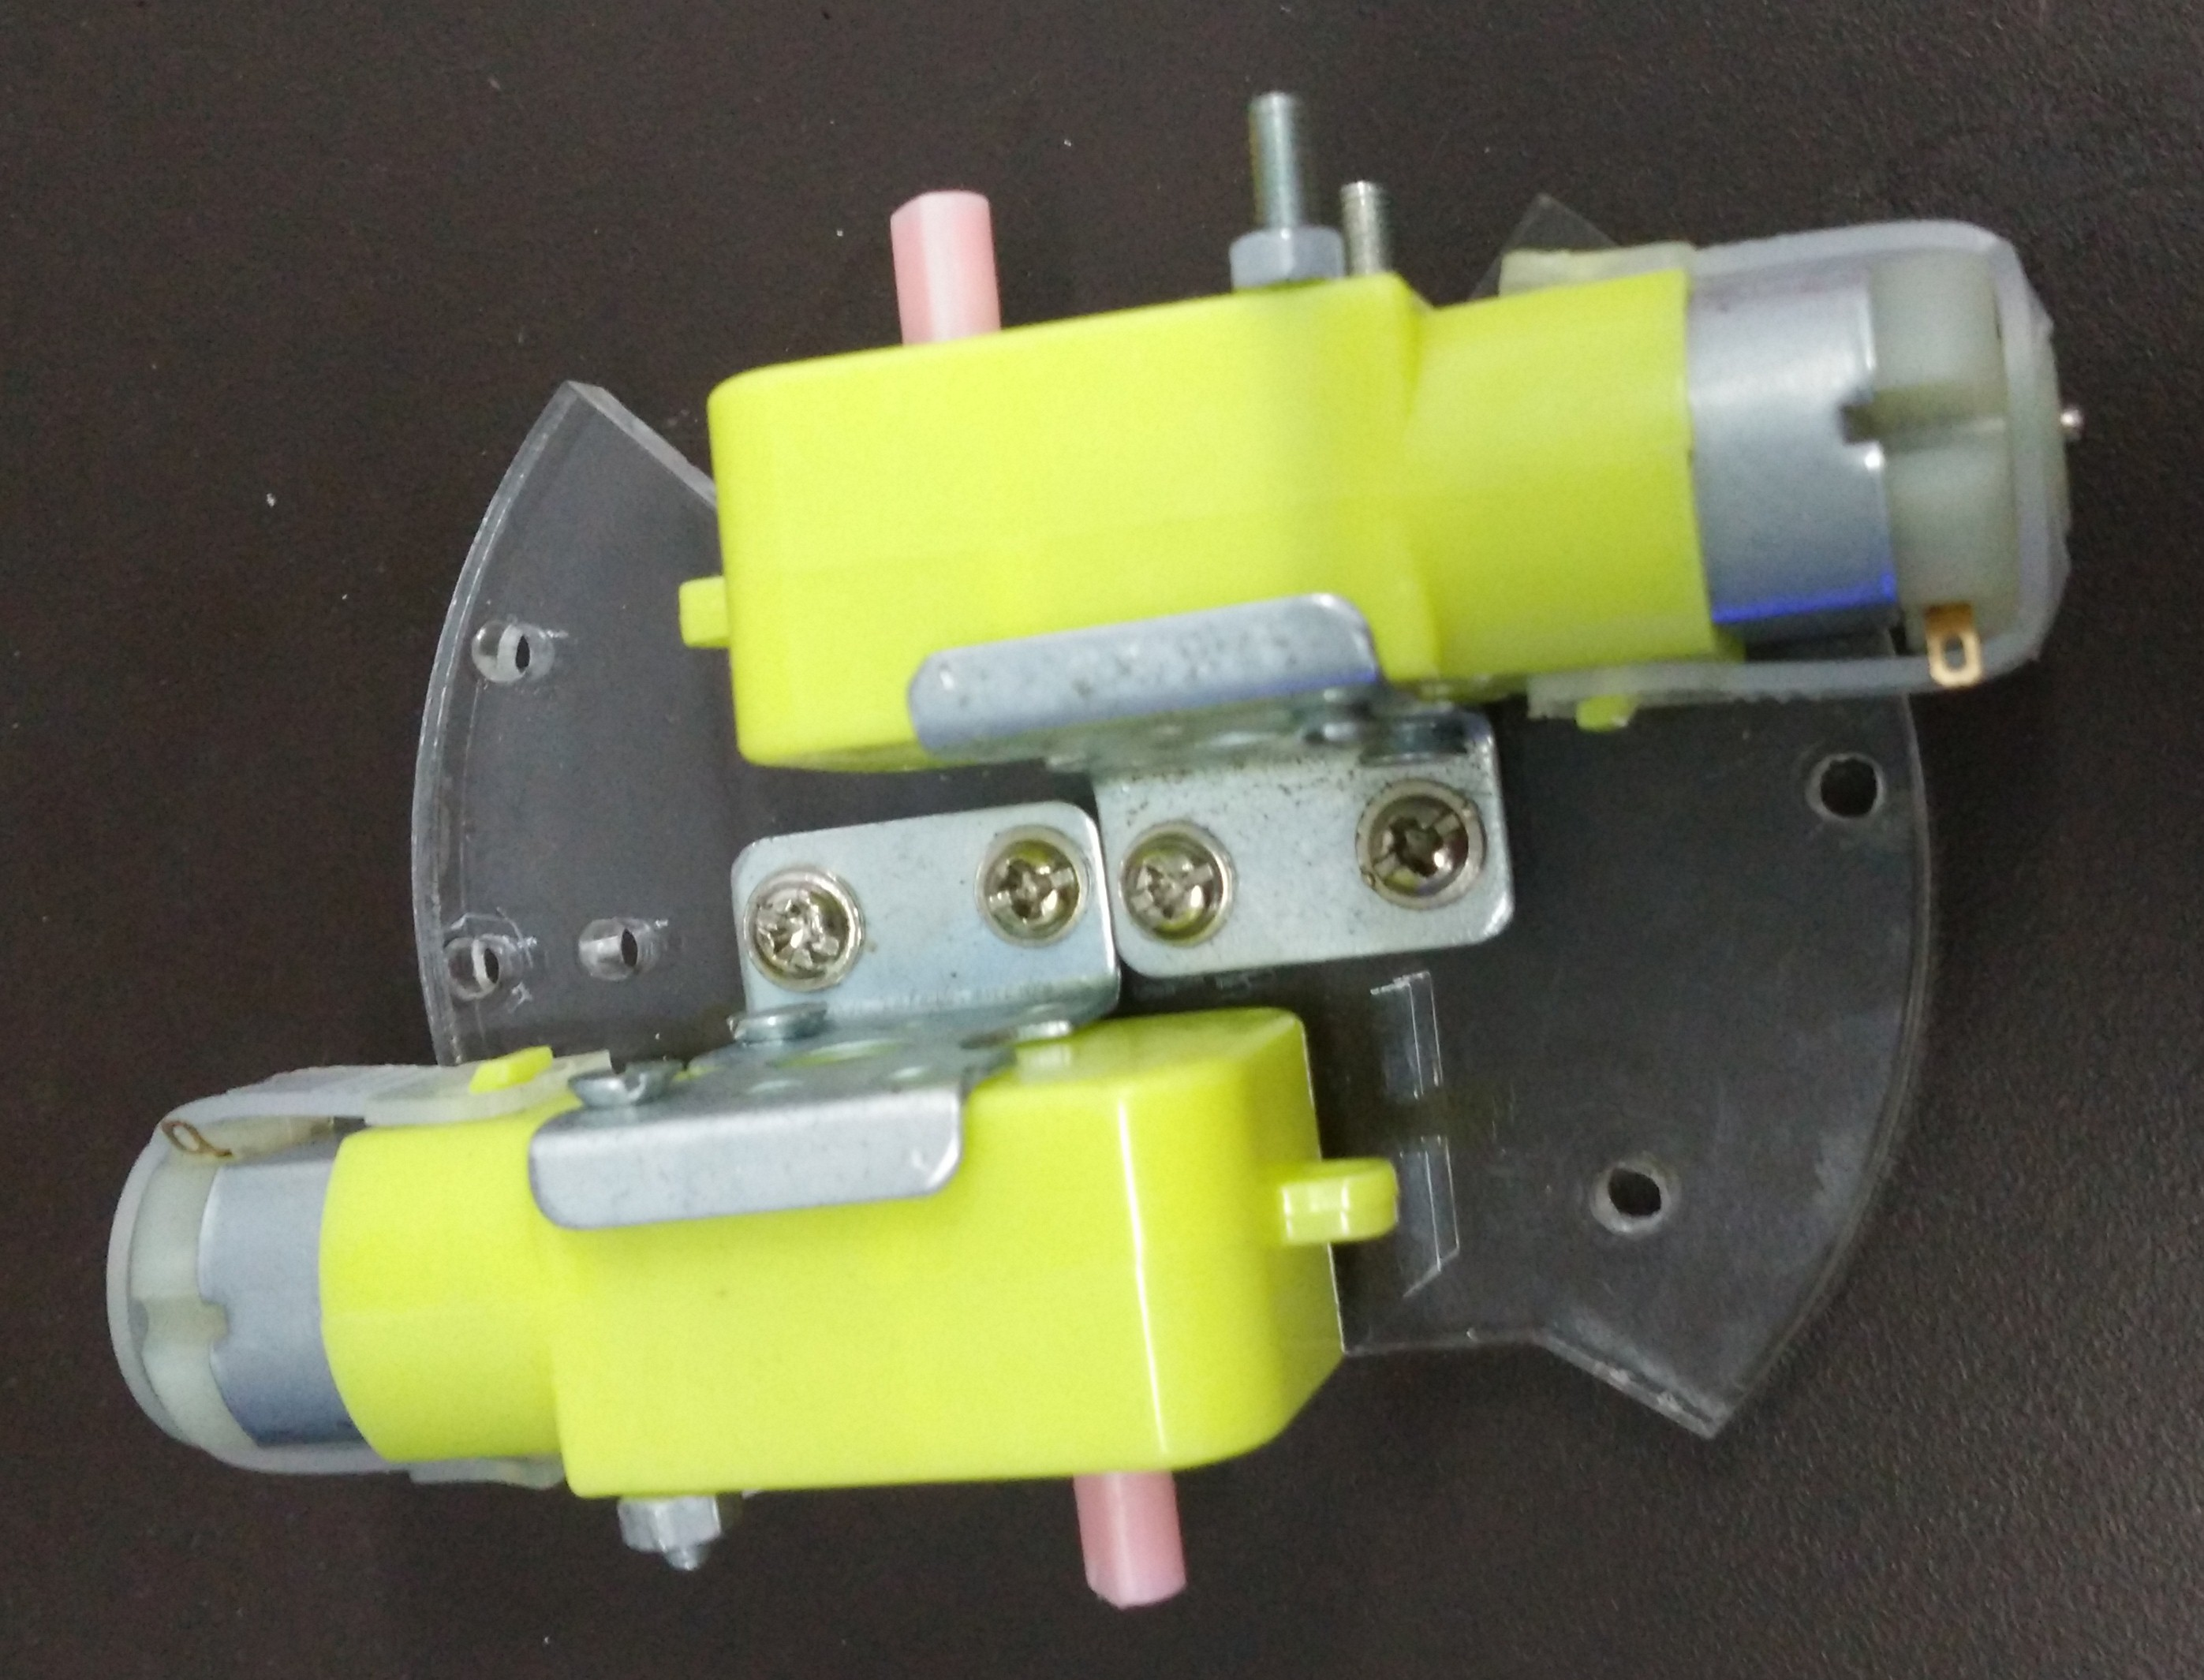
\includegraphics[width=350px]{./Pictures/Chassis_Design}		
\end{figure}	
\hfill\\
\newpage        
\subsection*{Step 3}
Soldering PCBs and attaching PCB on top of chassi.
\hfill\\
\begin{figure}[h!]
	\caption{Complete robot.}
	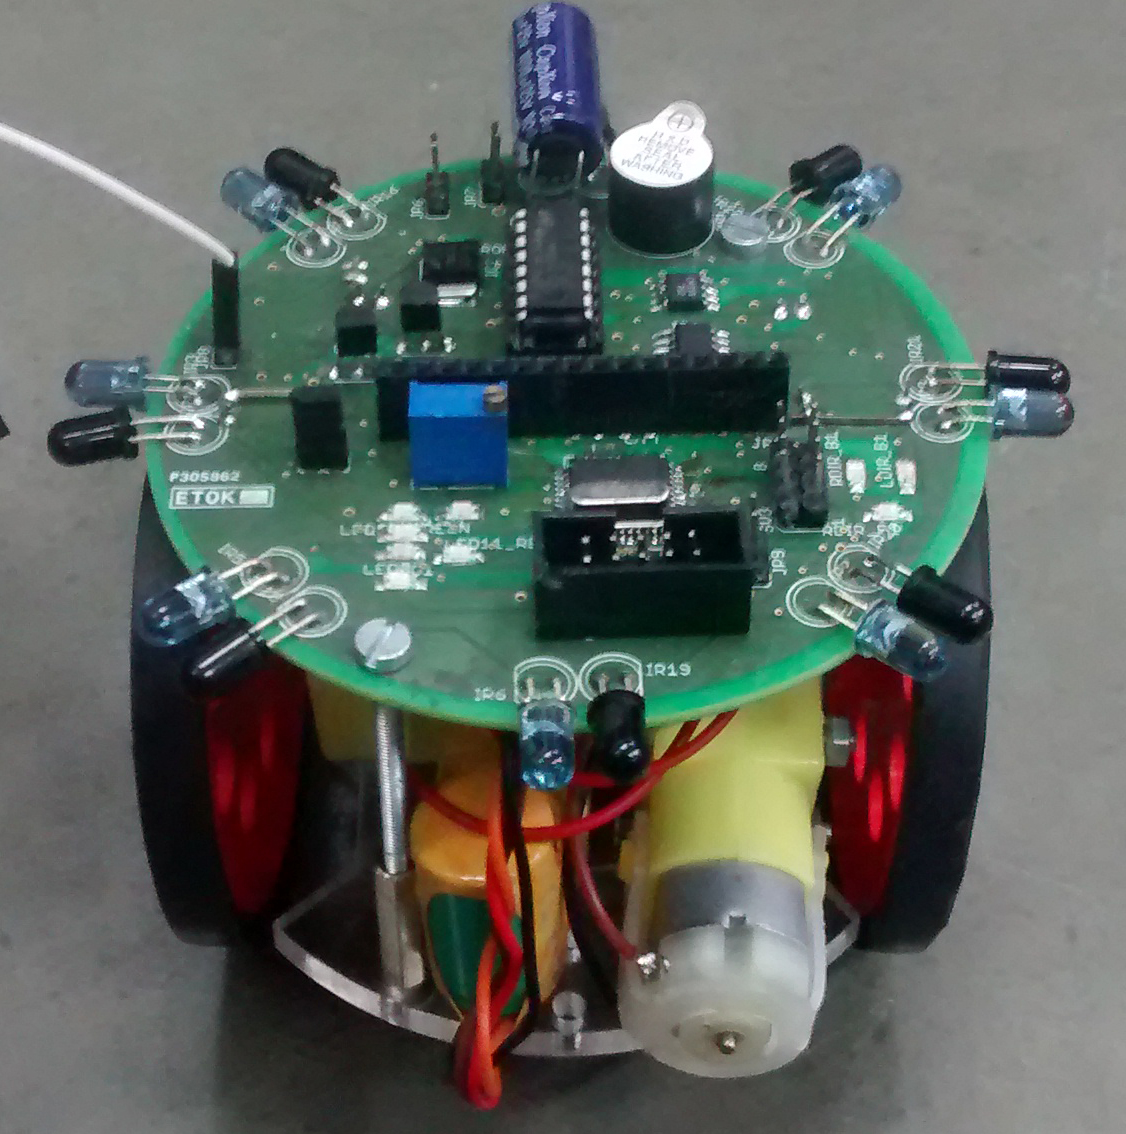
\includegraphics[width=\textwidth]{./Pictures/version2_top}		
\end{figure}	
\hfill\\
\newpage
\section{Software and Code}
\href{https://github.com/eYSIP-2017/eYSIP-2017_DistributedRobotics.git}{Github link} for the repository of code

\section{Use and Demo}
Final Setup Image

User Instruction for demonstration

\href{http://www.youtube.com}{Youtube Link} of demonstration video 

\section{Future Work}
Design an outer covering.\\
Implementing gathering and circle formation algorithms on Mini bots.\\
Solve collision of homogeneous dynamic swarm robots.\\

\section{Bug report and Challenges}
\hfill\\
	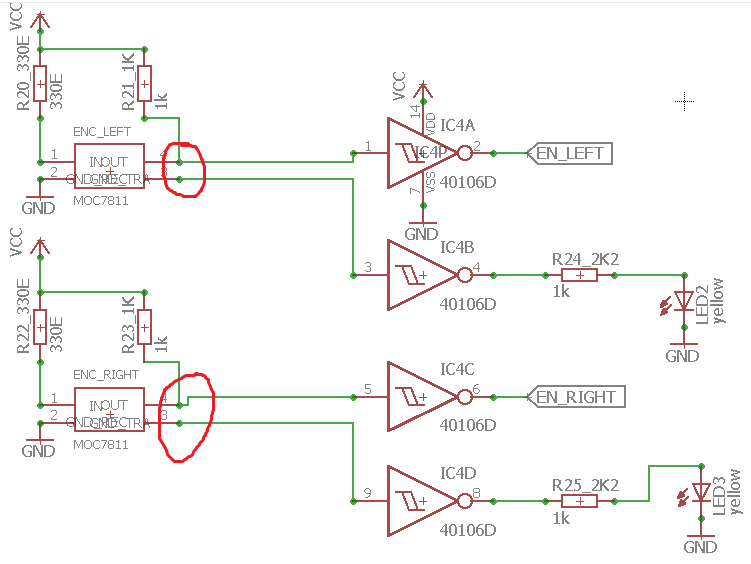
\includegraphics[width=\textwidth]{./Capture2.png}
\hfill\\

Bugs: Pin 3 of both encoders was supposed to be shorted to ground and connection to buffer connected to led was supposed to be shorted to pin 4.\\
Fix: The bug is fixed by shorting pin 3 to ground externally.\\

Challenges faced:\\
Placing components and routing air wires of PCB.\\

Reducing overall size of PCB.\\

Understanding different algorithms for circle formation and gathering algorithms for swarm robots to determine a common point for resolving global coordinate system\\

Soldering SMD components accurately.\\

\begin{thebibliography}{li}
\bibitem{wavelan97}
Ayan Dutta, Sruti Gan Chaudhuri, Suparno Datta and Krishnendu Mukhopadhyaya,
{\em Circle formation by asynchronous fat robots with limited visiblity}

\bibitem{wavelan97}
Sruti Gan Chaudhuri and Krishnendu Mukhopadhyaya,
{\em Gathering Asynchronous Transparent Fat Robots}

\bibitem{wavelan97}
Ayan Dutta, Sruti Gan Chaudhuri, Suparno Datta and Krishnendu Mukhopadhyaya,
{\em Circle formation by asynchronous fat robots}

\bibitem{wavelan97}
Swapnil Ghike and Krishnendu Mukhopadhyaya,
{\em A distributed algorithm for pattern formation by autonomous robots, with no agreement on coordinate compass}

\bibitem{wavelan97}
Avik Chatterjee, Sruti Gan Chaudhuri, Krishnendu Mukhopadhyaya,
{\em Gathering asynchronous swarm robots under non uniform limited visibilities}

\bibitem{wavelan97}
Krishnendu Mukhopadhyaya,
{\em Distributed swarm robotics for swarm robots}
\end{thebibliography}

\end{document}